%form: dc_form_05-07.tex ; user: dc_05-07_purpose_plan_rights.tex
%========== DC =========
%===== p. 05-07 研究の目的・内容、特色、計画、人権 =============
\subsection{研究の目的・内容}
%watermark: w02_purpose_plan_ugly_dc
\newcommand{\研究目的}{%
%begin  研究目的と内容===================
	\noindent
	●\textbf{研究目的}

	本研究では、SNS上でフェイクニュースの拡散を抑制するために、早期自動検出の精度向上と説明可能性の付与を目的とする。
	具体的には、(1)\textbf{生成されたコメントを使用した分類でF値が0.8を上回る手法の確立}と、
	(2)\textbf{生成されたコメントからユーザへ説明可能性を提案する手法の確立}を目指す研究を行う。

	\noindent
	●\textbf{研究方法・研究内容}

	\noindent
	(1) 生成されたコメントを使用した分類でF値が0.8を上回る手法の確立: 

	早期発見できてもユーザから信用が得られない狼少年的なモデルではなく、
	\textbf{的確にフェイクニュースだけを発見させることが可能なモデル}を構築する。
	また、性能向上に向く大規模データセットがない場合は条件に符合するものを自作する。
	最低でもF値0.7以上を目指す。

	\noindent
	(2)生成されたコメントからユーザへ説明可能性を提案する手法の確立:

	SNS上でフェイクニュースの疑いが強い指摘をする場合を想定し、\textbf{生成したコメントを理由付けの題材として活用する}ことを目指す。
	また、\textbf{理由付けの有無によってSNS利用者からの信用を得られる}ことを主観実験で示す。
	生成コメントから理由付けが難しいならば、実投稿からの実現を目指す。

	\noindent
	●\textbf{所属研究室との関連}

	当研究室はエージェント、知的Web、ソフトウェア工学、データマイニングの4つの分野に渡っており、
	本研究はデータマイニングの一環となる。
	また、デマや噂の検出を含めても本研究には前例はなく、\textbf{申請者が当研究室で初めて本研究に着手}した。

	\noindent
	●\textbf{研究計画の期間中に異なった研究機関(外国の研究機関等を含む。)において研究に従事することを予定}
	
	申請者は\textbf{期間中1年間北米あるいは欧州の研究施設での活動を予定}している。
	国内外でフェイクニュース対策研究には温度差が見られ、特に北米と欧州では盛んに研究が行われている(次項目で詳説)ことから、
	\textbf{最前線の研究に従事する}ためにも申請者が現地で研究に従事することが必要である。

%end  研究目的と内容 ====================
}

\newcommand{\人権の保護及び法令等の遵守への対応}{%
%begin  人権の保護及び法令等の遵守への対応 ===================
	コメント取得を予定してしているSNSはTwitterである。
	Twitter社は2020年3月より学術目的でTwitter APIの利用を自由化しているほか、
	取得したツイートIDを含む情報をデータセットとして公開することも学術目的であれば認められている\cite{twitter_2020}。

	また、先行研究が提供したデータセットを使用する場合は、提供者が示すライセンスやポリシーを遵守する。

	なお、学習済みモデルの公表は平成30年改正著作権法第30条4号により認められている。


	{\small
		\begin{thebibliography}{99}
			\setcounter{enumiv}{9}
			\bibitem{twitter_2020} Twitter開発者ポリシーを分かりやすくアップデート, 2020年3月11日. (最終閲覧日 2020年4月19日) \url{https://blog.twitter.com/developer/ja_jp/topics/tools/2020/DevPolicyUpdate.html}
		\end{thebibliography}
	}
%end  人権の保護及び法令等の遵守への対応 ====================
}

\newcommand{\研究の特色と独創的な点tillNextPage}{%
%begin  研究の特色と独創的な点===================
	\noindent
	●\textbf{これまでの先行研究等があれば、それらと比較して、本研究の特色、着眼点、独創的な点}

	ニュースに寄せられそうなコメントを生成する手法は、
	確率分布に従った潜在変数と正解ラベルを使用して頻出単語を生成するTCNN-URGが提案されている\cite{ijcai2018-533}。
	本研究は\textbf{頻出単語を生成するのではなく}、説明可能性に繋ぎやすい\textbf{実際に投稿されたようなコメントを生成する}ことを目指している。

	また、速報性を維持するためにユーザの反応を補完する弱教師あり学習を活用した手法であるMWSSも既に今年提案されている\cite{Shu2020LeveragingMW}。
	本研究では\textbf{生成する対象をコメントに絞っている}。
	他のユーザの反応(リツイート、いいね、反応したユーザ情報)はコメントに比べて説明可能性に繋げにくいためである。

	フェイクニュース対策に説明可能性を提供する手法として、
	記事とコメントから真偽判断の決め手となった部分を評価するdEFENDが提案されている\cite{shu2019defend}。
	これは既に投稿されたコメントを対象に含むため、まだコメントが多く寄せられていない状況である\textbf{早期発見を目指す場合には向かない}。
	当研究では、\textbf{生成されたコメントから説明可能性を提供する}ことで早期発見を実現する。

	\noindent
	●\textbf{国内外の関連する研究の中での当該研究の位置づけ、意義}

	風評やデマの自動検出も当該研究に含めると、歴史は決して浅くない。
	ただし、ここ\textbf{数年で社会情勢の変化によって一気に世界的に競争が激化}した。

	例えば、Google Scholar上で2015年に投稿された中で``fake news''でヒットする論文は\textbf{520本}に対して、
	同じ条件で2019年に投稿された論文は\textbf{15,400本}と実に\textbf{30倍近くに増加}した。

	前項目の通り、特に北米や欧州から頻繁に英語論文が発表されている。
	先述と同じプラットフォームで2019年で``フェイクニュース''でヒットする論文は\textbf{169本}と、1年間で実に日本語の\textbf{90倍以上}の英語論文が発表されている。

	これは\textbf{地域による問題意識の差}の他にも、特に(本研究を含め)近年機械学習やDNNを活用した研究が多いことも考えられる。
	これらの手法に必要な記事と真偽データなどを含む\textbf{大規模データセットが英語に集中している}のである。
	フェイクニュース検出の場合、ファクトチェック結果をラベル付けに流用することができるが、
	北米・欧州に比べて日本国内のファクトチェックは発展途上であるため、日本語データセットが少ない。
	もしも日本語を研究対象に含める場合、まずはデータセット作りから着手する必要がある。

	\noindent
	●\textbf{本研究が完成したとき予想されるインパクト及び将来の見通し}

	本研究が完成すると、SNSの利用者へこの情報が事実かフェイクかを判断する新しい判断材料を早い段階からもたらすことができる。
	また、フェイクニュースがSNS上で\textbf{早い段階で説得力がある理由によって指摘}することにより、
	利用者による\textbf{拡散を抑制}することができる。
	古今東西で虚偽情報を流布しようとする人々は存在するが、\textbf{利用者が簡単に騙されないような仕組み作り}を行うことで、
	\textbf{ジャーナリズムと民主主義に対する最大の脅威であるフェイクニュースから人々を守る}ことが可能となる。
	
	{\small
		\begin{thebibliography}{99}
			\setcounter{enumiv}{6}
			\bibitem{ijcai2018-533} Feng Qian, \textit{et al.} Neural user response generator: Fake news de-tection with collective user intelligence. In \textit{Proc. of the IJCAI-18}, pp. 3834–3840., 2018.
			\bibitem{Shu2020LeveragingMW} Kai Shu, \textit{et al.} Leveraging multi-source weak social supervision for early detection of fake news. \textit{arXiv}, Vol.abs/2004.01732, 2020.
			\bibitem{shu2019defend} Kai Shu, \textit{et al.} defend: Explainable fake news detection. In \textit{Proc. of the ACM SIGKDD}, 2019.
		\end{thebibliography}
		%\bibliography{myreferences}
		%\bibliographystyle{junsrt}
	}
%end  研究の特色と独創的な点 ====================
}

\newcommand{\研究計画withVspaceDC}{%
%begin  研究計画 ===================
	% 今年の様式は困ったものです。ブツブツ。
	% 今の技術では「(4)研究計画」のスタート位置を指定できることができません。
	% すみませんが、次の2行を調整してください。
%	\clearpage	% もし「(3) 研究の特色・独創的な点」がp.6に流れこまないなら、この行を有効にしてください。
	\vspace*{16mm}	% 「(4) 研究計画」が正しい高さから始まるように、この値を調整してください。

	%\textbf{この行の高さは、上の「研究の特色・独創的な点」との間隔を\textbackslash vspaceを用いて調整してください。}

	本研究の3年間のスケジュールを以下の表\ref{tbl:chart}に示す。

	\vspace*{-7mm}

    \begin{table}[h]
		\caption{本研究の年次計画(1セルは半期を表す)}
		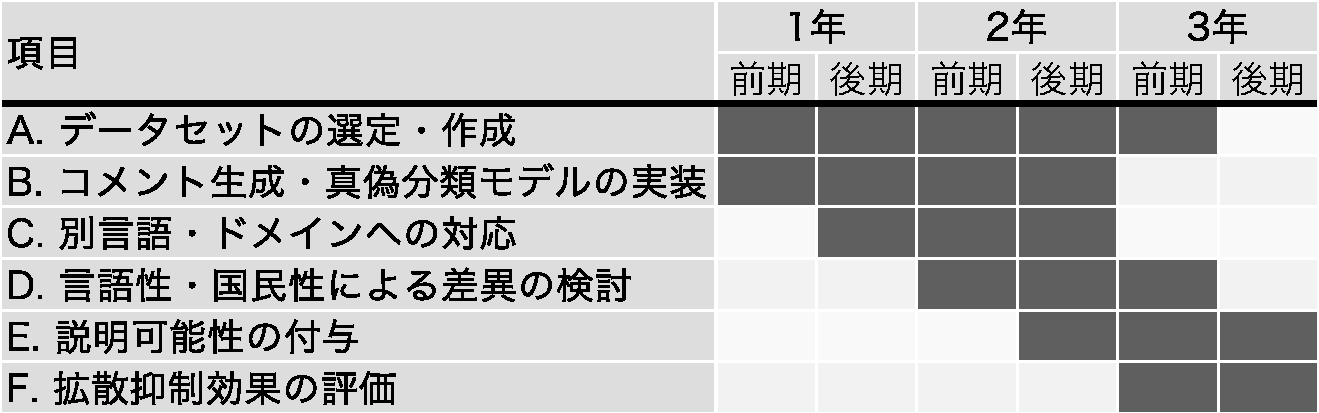
\includegraphics[width=\linewidth]{figs/chart.pdf}
		\label{tbl:chart}
    \end{table}
	
	\vspace*{-9mm}

	\noindent
	●\textbf{1年目}

	\noindent
	\textbf{A. データセットの選定・作成}

	以下の各タスクで使用するデータセットを随時選定する。
	条件はタスクによるが、例えばBならニュースとその真偽、そしてユーザのコメントである。
	もしも条件を満たすデータセットがない場合は、データセットを自分で集める必要がある。	

	\noindent
	\textbf{B. コメント生成・真偽分類モデルの実装}

	コメントを生成し分類するモデルの実装を引き続き行う。
	もしも現有モデルの拡張では難しい場合は別の手法からの拡張も検討している。

	\noindent
	\textbf{C. 真偽分類性能向上}

	本研究では生成コメントを含めた真偽判定において、分類の総合指標であるF値が0.8を上回ることを目指している。
	データセットの規模拡大やパラメータの調整、分類モデルの変更などで実現を目指す。

	\noindent
	●\textbf{2年目}

	\noindent
	\textbf{D. 別言語・ドメインへの対応}

	言語やニュースのトピックであるドメインの変動に提案モデルを対応させる。
	特に日本語対応する場合、形態素解析や事前学習済み日本語単語の分散表現の用意が必要である。
	また、いずれも同時にデータセットも新たに用意しなければならない。

	\noindent
	\textbf{E. 説明可能性の付与}

	ユーザに説明可能性を提供するために、生成されたコメントから真偽を判断した材料を取得する。
	これは分類モデルを拡張することによって実現が可能であると考えている。

	\noindent
	●\textbf{3年目}

	\noindent
	\textbf{F. 拡散抑止力の評価}

	実際にSNS上で提供した時を想定し、分類成績を改善させ説明可能性を付与したモデルがSNS利用者への意識にどのような影響を与えるか主観評価実験によって評価する。
	もしも生成されたコメントから説明可能性が得られない場合は、実際に投稿されたコメントや記事から得ることを予定している。


%end  研究計画 ====================
}

